\chapter{Análise Filogenética através de Redes Complexas} \label{cap:analisefilo}

Análise Filogenética é uma área da Biologia que tem despertado bastante interesse pelos pesquisadores. A evolução do poder de processamento dos computadores
permitiu que se pudesse comparar sequências proteicas ou nucleotídicas muito rapidamente, gerando um poder de análise abrangente no que tange as relações entre
proteinas, enzimas, rotas metabólicas e consequentemente seres vivos. Essas análises, por conseguinte, geraram descobertas importantes que influenciaram o
modo como enxergamos a evolução das espécies e a relação entre elas em geral.

Atualmente existem quatro métodos bem aceitos na literatura para Análise Filogenética: Análise Bayesiana \textbf{[CITAR]}, Análise de Parcimônia
\textbf{[CITAR]}, Análise de Distâncias \textbf{[CITAR]} e Análise por Verossimilhança \textbf{[CITAR]}. Estas análises partem de alguns pressopostos
biológicos, que são informações iniciais necessárias a sua realização. O uso da Física Estatística para tratar os dados referentes a proteinas de
determinadas rotas metabólicas permite o desenvolvimento de um método que não necessite desses pressupostos.

A área de Física Estatística atualmente apresenta forte caráter interdisciplinar, permitindo a modelagem e análise de diversos sistemas
que englobam outras áreas de conhecimento. A aplicação da Teoria das Redes Complexas em Bioinformática, apoiada pela Teoria dos Grafos,
juntamente com conhecimentos de Física, Matemática e Biologia vem se mostrando como uma alternativa interessante na modelagem de sistemas biológicos,
e serviu para que o FESC (Física Estatística e Sistemas Complexos - Instituto de Física - UFBA) desenvolvesse um método para Análise Filogenética.

\sigla{FESC}{Física Estatística e Sistemas Complexos - Instituto de Física - UFBA}

Como foi dito anteriormente, o objetivo deste trabalho é controlar o processo e fornecer um ambiente para o armazenamento de informações em relação às
execuções, além de uma interface de fácil utilização para um pesquisador da área de Biologia. A figura \ref{fig:fluxograma} mostra o fluxograma geral
sobre os passos da execução do método. As seções que seguem explicam estes passos com mais detalhes.

\begin{figure}
\centering

\includegraphics{brasaoUFBA2}
\caption{Fluxograma com os passos da execução do método de análise filogenética desenvolvido pelo FESC.}
\label{fig:fluxograma}
\end{figure}


\section{Escolha de Sequências Proteicas} \label{sec:escseq}

A primeira etapa do método consiste na escolha das sequências que serão utilizadas para a construção e caracterização da rede.
Usualmente a escolha é feita a partir de um banco de dados biológico, disponível livremente pela web. Durante todo o trabalho na utilização
do método, as sequências escolhidas vieram do NCBI \cite{ncbi}, um banco de dados bastante utilizado no meio biológico, que contém dados de sequências
nucleotídicas e sequências proteicas, entre várias outras informações. A escolha das sequências proteicas é feita utilizando como critério
uma rota metabólica, separando as sequências pela enzima que as produzem na rota.

\sigla{NCBI}{National Center for Biotechnology Information}

Esta é uma etapa manual, onde são feitas buscas por data e são realizadas determinadas filtragens no site do NCBI para obter as sequências desejadas. O
sistema desenvolvido neste trabalho leva em consideração que as sequências já foram escolhidas e as recebe como entrada inicial. O resultado desta etapa
são arquivos no formato GenBank (NCBI) que são filtrados e organizados para facilitar a identificação de organismos em etapas posteriores e proporcionar
a execução da similaridade.

\section{Similaridade} \label{sec:similaridade}

Para executar a similaridade, primeiro os dados no formato GenBank são filtrados e armazenados em um banco de dados relacional. Então é utilizado o BLAST
(Basic Alignment Search Tool) \cite{blast1997} para comparação entre as sequências. O BLAST trabalha tanto com sequências nucleotídicas quanto proteicas.
O interesse do uso do BLAST para o método em questão está na comparação de sequências proteicas utilizando o alinhamento local, que compara duas sequências
isoladamente e retorna uma porcentagem de similaridade entre elas.

\sigla{BLAST}{Basic Alignment Search Tool}

A partir do resultado do BLAST, pode-se construir uma matriz de similaridades \cite{andrade2006}, onde as linhas e colunas são as sequências e
a relação é a similaridade entre elas. Desta matriz são construídas as redes que caracterizam as sequências, que serão descritas na próxima seção.

\section{Construção e Caracterização das Redes} \label{sec:conscarac}

O conceito de rede está associado ao de um grafo. É um conjunto de vértices e arestas conectando-os. Podemos dizer que o estudo de uma rede é o
estudo de um grafo, mas em uma escala maior. Redes podem ser tidas como grafos muito grandes e complexos, em que se torne mais preciso o uso de
técnicas estatísticas para a sua análise \cite{bessa2008}. Na literatura de Redes Complexas, em geral, precisamos encontrar uma rede de determinado
conjunto que melhor caracterize este conjunto. Essa escolha se dá pela relação entre ruído e informação \cite{barabasi2004}.

Partindo da matriz de similaridades, podemos construir até 101 matrizes de adjacência, se levarmos em consideração que podemos escolher um valor
limiar e construir a rede baseada nele. Por exemplo, se escolhermos o valor 60 como limiar, construiremos uma rede onde haverá uma aresta aresta entre
dois vértices (sequências) se e somente se a similaridade entre eles em questão for maior ou igual a 60. Uma rede com limiar muito baixo apresenta muito
ruído e uma rede com limiar muito alto apresenta pouca informação.

Partindo das matrizes de adjacência podemos também criar matrizes de vizinhança \cite{andrade2009}, que podem ser obtidas calculando-se os caminhos mínimos
\cite{bessa2008} entre os vértices da rede ou através da multiplicação booleana de matrizes de adjacência de ordens consecutivas \cite{andrade2006}. Na figura 
\ref{fig:matriz-vizinhanca}, temos um exemplo de matriz de vizinhança (com os números em forma de cor).

\begin{figure}
\centering
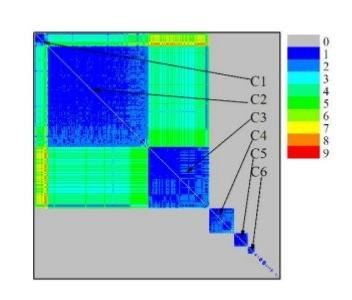
\includegraphics[scale=0.53]{matriz-vizinhanca}
\caption{Exemplo de Matriz de Vizinhança no formato de Matriz de Cores.}
\label{fig:matriz-vizinhanca}
\end{figure}

Para a execução desta etapa, é utilizado o programa \textit{Rede Crítica}, desenvolvido na linguagem Fortran. As matrizes de vizinhança são importantes para
etapas posteriores do processo, inclusive a etapa seguinte, que é a determinação do limiar crítico.

\section{Limiar Crítico} \label{sec:limcrit}

Já se sabe que o limiar crítico de uma rede revela a melhor relação entre ruído e informação. Existem diversas maneiras de se determinar o limiar
crítico da rede. Uma delas, utilizada pelo FESC, é o método das distâncias \textbf{[CITAR REFERÊNCIA DO ARTIGO DA PLOS]}. Nele, calcula-se a
distância euclidiana entre matrizes de vizinhança de limiares consecutivos. A matriz que apresentar a maior distância entre a de limiar conscutivo
ao seu será a escolhida como a matriz do limiar crítico, para representar a rede. É necessário escolher a melhor rede que representa o conjunto.
A rede do limiar crítico cumpre bem este papel.

Para a execução desta etapa, é utilizado o programa \textit{Rede Crítica}, desenvolvido na linguagem Fortran. Na figura \ref{fig:distancia}, temos o
exemplo de um resultado do cálculo das distâncias entre matrizes de vizinhança, onde o limiar crítico é representado pelo pico do gráfico, ou seja,
o valor 51. A rede que representa todo o conjunto é então a rede do limiar 51, que será utilizada na última etapa do processo, que é a clusterização,
que utiliza um conceito chamado entremeação.

\begin{figure}
\centering
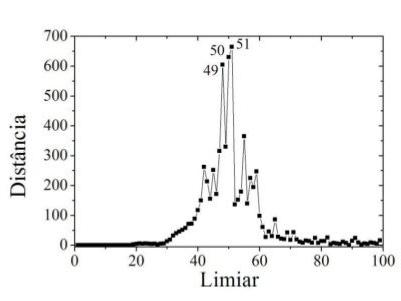
\includegraphics[scale=0.58]{distancia}
\caption{Resultado da execução do método das distâncias entre limiares consecutivos, resultando em um gráfico Distância x Limiar.}
\label{fig:distancia}
\end{figure}

\section{Entremeação e Centralidade} \label{sec:entremeacao}

A Matriz de Vizinhança da rede do limiar crítico é a entrada necessária para a realização da clusterização, que é feita através do método de detecção
de comunidades de Newman e Girvan \cite{newman2004} para identificar a estrutura modular da rede. O método consiste em determinar a aresta mais importante
da rede – aquela por onde passa a maior quantidade de caminhos mínimos de cada par de vértices por toda a rede – e eliminá-la, repetindo a operação
até que não existam mais arestas na rede.

Para a execução desta etapa, é utilizado o programa \textit{Dendo}, em Fortran. Conforme a operação é feita, é possível construir um histograma de remoção
de arestas (dendrograma), que auxilia na identificação de comunidades e propicia as análises biológicas dos resultados, além da comparação com outros
métodos da Biologia. A figura \ref{fig:dendrograma} mostra com detalhes um exemplo de dendrograma para o limiar crítico 51.\newline

\begin{figure}
\centering
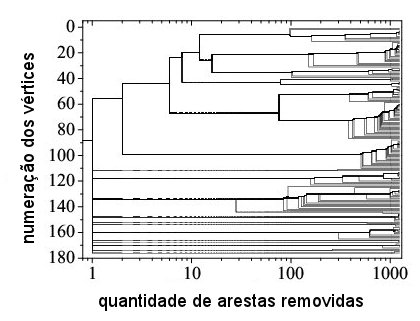
\includegraphics[scale=0.73]{dendrograma}
\caption{Exemplo de dendrograma para o limiar crítico 51.}
\label{fig:dendrograma}
\end{figure}

O método em questão utiliza uma determinada quantidade de programas, cada um seguindo certos padrões de entrada e saída, além de arquivos de configuração.
Tais características dificultam sua utilização por pesquisadores de outras áreas que não Física ou Ciência da Computação, além de trazê-los uma preocupação
desnecessária com localização e distribuição de arquivos. Para um melhor aproveitamento do método, seria mais interessante que o controle do processo de
execução fosse realizado por um sistema, dispondo de um ambiente de fácil utilização e que realizasse o gerenciamento das informações por meio de uma camada
de persistência, deixando a questão da organização dos dados transparente para o pesquisador.

A tabela \ref{tab:requisitos} mostra os requisitos necessários para a construção do Navi - Sistema para Gerenciamento de Informações e Execuções de Análise
Filogenética Através de Redes Complexas.

\begin{table}
\centering
\caption{Tabela de requisitos do Navi} % igual ao ambiente figura
\begin{tabular}{c} % com este comando dizemos quantas colunas terá nossa tabela e a posição do texto dentro de cada coluna. Aqui temos três colunas (pois são três "c" dentre {}) e o texto estará centralizado em todas elas (indicado pelo "c", se quisermos alinhados à esquerda "l" ou direita "r"
\hline 
%Requisito & Pontos & Classificação \\
Requisito \\ 
\hline
\hline
%Cruzeiro & 52 & 1 \\
%Sao Paulo & 50 & 2 \\
%Gremio Barueri & 47 & 3 \\
Criar novo projeto \\
Abrir projeto existente \\
Gerar matriz de adjacências de um limiar qualquer \\
Gerar matriz de vizinhança de um limiar qualquer \\
Visualizar o gráfico de matriz de vizinhança qualquer em forma de matriz de cores \\
Analisar limiares \\
Executar clusterização \\
Comparar/executar congruência de redes de diferentes projetos \\
Visualizar gráfico completo da rede \\
Executar congruência em relação a um arquivo cadastrado em um formato padrão \\
Exportar dados do projeto para gráficos em um formato de programas plotadores \\
\hline
\end{tabular}
\label{tab:requisitos}
\end{table} 

\chapter{Navi - Sistema para Gerenciamento de Informações e Execuções de Análise Filogenética Através de Redes Complexas}
\label{cap:navi}

\section{Escopo do Sistema} \label{sec:escopo}

bla

\section{Organização das Informações} \label{sec:organizacao}

bla

\section{Dinâmica do Sistema} \label{sec:dinamica}

bla


\chapter{Resultados}
\label{cap:resultados}


\section{Ambiente de execução} \label{sec:ambiente}

bla
troca de banco de dados relacional para serialização de objetos

\section{Ferramentas de Desenvolvimento} \label{sec:ferramentas}

bla

\section{Discussão} \label{sec:discussao}

bla

\section{Dificuldades} \label{sec:dificuldades}

bla



\section{Listagens} \label{sec:listagens}

Nonono nonnono onononono \cite{fowler2000}.

Na listagem \ref{lst:testjUnit} 
e mostrado o teste do metodo \texttt{Engine.initialize()}:

\lstset{language=java}
\lstset{commentstyle=\textit}
\begin{lstlisting}[frame=trbl, caption=Classe Factory2D,label=lst:testjUnit]{}
public class EngineTest
// JUnitDoclet begin extends_implements
extends TestCase
// JUnitDoclet end extends_implements
{
  //...
  public void testInitialize() throws Exception {
   // JUnitDoclet begin method initialize
   EngineState engineState = (EngineState) PrivateAccessor.
    getField(engine,"engineState");
   engine.initialize();
   assertEquals(engineState, new InitState());
   // JUnitDoclet end method initialize
  }
  ...
}
\end{lstlisting}

Como visto no capitulo \ref{cap:analisefilo}, no nonno\footnote{Isto e uma nota
de rodape.} no nonon onono:
\begin{itemize}
  \item{nononoo}
  \item{nononono}
  \item{no}
\end{itemize}


\section{Figuras} \label{sec:figuras}

E possivel usar imagens vetoriais no \cite{andrade2006} formato PDF, como pode ser visto
na figura \ref{fig:ufba}, ou imagens \emph{bitmap} no formato PNG, como
a da figura \ref{fig:ufba2}.

\begin{figure}
\centering

\includegraphics{brasaoUFBA2}
\caption{Brasao da UFBA (vetorial)}
\label{fig:ufba}
\end{figure}

\begin{figure}
\centering

\includegraphics[width=0.3\textwidth]{brasaoUFBA}
\caption{Brasao da UFBA (\emph{bitmap})}
\label{fig:ufba2}
\end{figure}
